\documentclass[
  man,
  floatsintext,
  longtable,
  nolmodern,
  notxfonts,
  notimes,
  mask,
  colorlinks=true,linkcolor=blue,citecolor=blue,urlcolor=blue]{apa7}

\usepackage{amsmath}
\usepackage{amssymb}




\RequirePackage{longtable}
\RequirePackage{threeparttablex}

\makeatletter
\renewcommand{\paragraph}{\@startsection{paragraph}{4}{\parindent}%
	{0\baselineskip \@plus 0.2ex \@minus 0.2ex}%
	{-.5em}%
	{\normalfont\normalsize\bfseries\typesectitle}}

\renewcommand{\subparagraph}[1]{\@startsection{subparagraph}{5}{0.5em}%
	{0\baselineskip \@plus 0.2ex \@minus 0.2ex}%
	{-\z@\relax}%
	{\normalfont\normalsize\bfseries\itshape\hspace{\parindent}{#1}\textit{\addperi}}{\relax}}
\makeatother




\usepackage{longtable, booktabs, multirow, multicol, colortbl, hhline, caption, array, float, xpatch}
\setcounter{topnumber}{2}
\setcounter{bottomnumber}{2}
\setcounter{totalnumber}{4}
\renewcommand{\topfraction}{0.85}
\renewcommand{\bottomfraction}{0.85}
\renewcommand{\textfraction}{0.15}
\renewcommand{\floatpagefraction}{0.7}

\usepackage{tcolorbox}
\tcbuselibrary{listings,theorems, breakable, skins}
\usepackage{fontawesome5}

\definecolor{quarto-callout-color}{HTML}{909090}
\definecolor{quarto-callout-note-color}{HTML}{0758E5}
\definecolor{quarto-callout-important-color}{HTML}{CC1914}
\definecolor{quarto-callout-warning-color}{HTML}{EB9113}
\definecolor{quarto-callout-tip-color}{HTML}{00A047}
\definecolor{quarto-callout-caution-color}{HTML}{FC5300}
\definecolor{quarto-callout-color-frame}{HTML}{ACACAC}
\definecolor{quarto-callout-note-color-frame}{HTML}{4582EC}
\definecolor{quarto-callout-important-color-frame}{HTML}{D9534F}
\definecolor{quarto-callout-warning-color-frame}{HTML}{F0AD4E}
\definecolor{quarto-callout-tip-color-frame}{HTML}{02B875}
\definecolor{quarto-callout-caution-color-frame}{HTML}{FD7E14}

%\newlength\Oldarrayrulewidth
%\newlength\Oldtabcolsep


\usepackage{hyperref}




\providecommand{\tightlist}{%
  \setlength{\itemsep}{0pt}\setlength{\parskip}{0pt}}
\usepackage{longtable,booktabs,array}
\usepackage{calc} % for calculating minipage widths
% Correct order of tables after \paragraph or \subparagraph
\usepackage{etoolbox}
\makeatletter
\patchcmd\longtable{\par}{\if@noskipsec\mbox{}\fi\par}{}{}
\makeatother
% Allow footnotes in longtable head/foot
\IfFileExists{footnotehyper.sty}{\usepackage{footnotehyper}}{\usepackage{footnote}}
\makesavenoteenv{longtable}

\usepackage{graphicx}
\makeatletter
\newsavebox\pandoc@box
\newcommand*\pandocbounded[1]{% scales image to fit in text height/width
  \sbox\pandoc@box{#1}%
  \Gscale@div\@tempa{\textheight}{\dimexpr\ht\pandoc@box+\dp\pandoc@box\relax}%
  \Gscale@div\@tempb{\linewidth}{\wd\pandoc@box}%
  \ifdim\@tempb\p@<\@tempa\p@\let\@tempa\@tempb\fi% select the smaller of both
  \ifdim\@tempa\p@<\p@\scalebox{\@tempa}{\usebox\pandoc@box}%
  \else\usebox{\pandoc@box}%
  \fi%
}
% Set default figure placement to htbp
\def\fps@figure{htbp}
\makeatother


% definitions for citeproc citations
\NewDocumentCommand\citeproctext{}{}
\NewDocumentCommand\citeproc{mm}{%
  \begingroup\def\citeproctext{#2}\cite{#1}\endgroup}
\makeatletter
 % allow citations to break across lines
 \let\@cite@ofmt\@firstofone
 % avoid brackets around text for \cite:
 \def\@biblabel#1{}
 \def\@cite#1#2{{#1\if@tempswa , #2\fi}}
\makeatother
\newlength{\cslhangindent}
\setlength{\cslhangindent}{1.5em}
\newlength{\csllabelwidth}
\setlength{\csllabelwidth}{3em}
\newenvironment{CSLReferences}[2] % #1 hanging-indent, #2 entry-spacing
 {\begin{list}{}{%
  \setlength{\itemindent}{0pt}
  \setlength{\leftmargin}{0pt}
  \setlength{\parsep}{0pt}
  % turn on hanging indent if param 1 is 1
  \ifodd #1
   \setlength{\leftmargin}{\cslhangindent}
   \setlength{\itemindent}{-1\cslhangindent}
  \fi
  % set entry spacing
  \setlength{\itemsep}{#2\baselineskip}}}
 {\end{list}}
\usepackage{calc}
\newcommand{\CSLBlock}[1]{\hfill\break\parbox[t]{\linewidth}{\strut\ignorespaces#1\strut}}
\newcommand{\CSLLeftMargin}[1]{\parbox[t]{\csllabelwidth}{\strut#1\strut}}
\newcommand{\CSLRightInline}[1]{\parbox[t]{\linewidth - \csllabelwidth}{\strut#1\strut}}
\newcommand{\CSLIndent}[1]{\hspace{\cslhangindent}#1}


\usepackage[nolongtablepatch]{lineno}
\linenumbers



\usepackage{fontspec} 

\defaultfontfeatures{Scale=MatchLowercase}
\defaultfontfeatures[\rmfamily]{Ligatures=TeX,Scale=1}

  \setmainfont[,RawFeature={fallback=mainfontfallback}]{Roboto}




\title{Preferences for costly cooperation are highly individualized}


\shorttitle{Costly cooperation}


\usepackage{etoolbox}









\authorsnames[{1},{1},{1},{2},{3},{2},{4,5},{6},{7,8},{1}]{Mikayla
Lalli,Nour Al Afif,Jiaqiao Tang,Hibaa Hasan,Enuri Dissanayake,Vida
Sussman,Rakshith Lokesh,Scott Rathwell,Joshua G.A. Cashaback,Michael J.
Carter}







\authorsaffiliations{
{Department of Kinesiology, McMaster University},{Department of
Psychology, Neuroscience \& Behaviour, McMaster University},{School of
Interdisciplinary Science, McMaster University},{Department of Biology,
Northeastern University},{Department of Electrical and Computer
Engineering, Northeastern University},{Department of Kinesiology \&
Physical Education, University of Lethbridge},{Department of Biomedical
Engineering, University of Delaware},{Department of Mechanical
Engineering, University of Delaware}}




\leftheader{Lalli, Afif, Tang, Hasan, Dissanayake, Sussman, Lokesh, Rathwell, Cashaback and Carter}



\abstract{When deciding between action alternatives, we use information
about the costs and rewards of each action to choose an appropriate
plan. Curioni et al. (\citeproc{ref-curioni2022}{2022}) recently found
that participants had a strong preference for completing a virtual
box-clearing task cooperatively with a partner rather than alone,
despite it being more motorically and cognitively costly. Participants
completed the task standing beside each other in close proximity, which
may have created a social pressure to cooperate through a need to manage
one's reputation or a sense of commitment. Here, 50 human pairs---each
composed of a ``Decision-maker'' and ``Helper''---completed a
box-clearing task modeled after Curioni et al.~while seated farther away
and out of view of one another. In 50\% of trials, Decision-makers were
forced to complete the task alone or with the Helper. In the remaining
50\% of trials, Decision-makers chose to work alone or cooperatively.
When working together, participants were required to synchronize their
movements without communication or feedback of their partner's
movements. Decision-makers answered open-ended questions regarding why
and when they chose to complete the task alone and together. We found a
slight preference for individual action over costly joint action, yet
this preference was not significantly different from chance. Inductive
thematic analysis revealed two dominant themes: ``chose actions with
greater instrumental utility'' and ``chose actions with greater social
value''. The identified themes suggest that preferences to cooperate are
highly individualized, and that cooperative actions may provide
additional social rewards that drive preferences for cooperation even
when it is more costly. }

\keywords{joint action, social decision-making, utility, costs, thematic
analysis}

\authornote{\par{\addORCIDlink{Mikayla
Lalli}{0000-0003-2589-7216}}\par{\addORCIDlink{Nour Al
Afif}{0009-0006-8948-8795}}\par{\addORCIDlink{Jiaqiao
Tang}{0009-0003-0265-4569}}\par{\addORCIDlink{Rakshith
Lokesh}{0000-0001-8592-5392}}\par{\addORCIDlink{Scott
Rathwell}{0000-0001-8775-1664}}\par{\addORCIDlink{Joshua G.A.
Cashaback}{0000-0002-8642-6648}}\par{\addORCIDlink{Michael J.
Carter}{0000-0002-0675-4271}} 
\par{ }
\par{   The authors have no conflicts of interest to disclose. This work
was supported by the Natural Sciences and Engineering Research Council
(NSERC) of Canada (RGPIN-2018-05589; MJC), McMaster University (MJC),
and the National Science Foundation (NSF: 2146888; JGAC). We thank
Dr.~Arianna Curioni for methodological clarifications about their
protocol when we were programming our version of the box-clearing
task.  Author roles were classified using the Contributor Role Taxonomy (CRediT; https://credit.niso.org/) as follows: Mikayla
Lalli:   Conceptualization, Data curation, Formal
analysis, Investigation - Performed the experiment, Methodology, Project
administration, Software - Task
Programming, Supervision, Validation, Visualization, Writing - Original
Draft Preparation, Writing - Review \& Editing; Nour Al
Afif:   Conceptualization, Investigation - Performed the
experiment, Methodology, Writing - Review \& Editing; Jiaqiao
Tang:   Conceptualization, Formal analysis, Investigation - Performed
the experiment, Methodology, Writing - Review \& Editing; Hibaa
Hasan:   Investigation - Performed the experiment, Writing - Review \&
Editing; Enuri Dissanayake:   Investigation - Performed the
experiment, Writing - Review \& Editing; Vida Sussman:   Investigation -
Performed the experiment, Writing - Review \& Editing; Rakshith
Lokesh:   Methodology, Software - Task Programming, Writing - Review \&
Editing; Scott Rathwell:   Conceptualization, Methodology, Writing -
Review \& Editing; Joshua G.A. Cashaback:   Conceptualization, Funding
acquisition, Methodology, Supervision, Writing - Original Draft
Preparation, Writing - Review \& Editing; Michael J.
Carter:   Conceptualization, Data curation, Formal analysis, Funding
acquisition, Methodology, Project
administration, Supervision, Validation, Visualization, Writing -
Original Draft Preparation, Writing - Review \& Editing}
\par{Correspondence concerning this article should be addressed
to Michael J. Carter, Department of Kinesiology, McMaster
University, 1280 Main Street West, Hamilton, ON L4S
4K1, Canada, Email: cartem11@mcmaster.ca}
}

\makeatletter
\let\endoldlt\endlongtable
\def\endlongtable{
\hline
\endoldlt
}
\makeatother

\urlstyle{same}


\usepackage[sfdefault,light]{roboto}
\usepackage{caption}
\usepackage{setspace}
\captionsetup[figure]{font=doublespacing,justification=justified}
\captionsetup[table]{font=doublespacing}
\usepackage{csquotes}
\MakeOuterQuote{"}
\raggedbottom
\usepackage{hyperref}
\hypersetup{
  hidelinks,
  colorlinks=false,
  }
\urlstyle{same}

\usepackage{booktabs}
\usepackage{longtable}
\usepackage{array}
\usepackage{multirow}
\usepackage{wrapfig}
\usepackage{float}
\usepackage{colortbl}
\usepackage{pdflscape}
\usepackage{tabu}
\usepackage{threeparttable}
\usepackage{threeparttablex}
\usepackage[normalem]{ulem}
\usepackage{makecell}
\usepackage{xcolor}
\makeatletter
\@ifpackageloaded{caption}{}{\usepackage{caption}}
\AtBeginDocument{%
\ifdefined\contentsname
  \renewcommand*\contentsname{Table of contents}
\else
  \newcommand\contentsname{Table of contents}
\fi
\ifdefined\listfigurename
  \renewcommand*\listfigurename{List of Figures}
\else
  \newcommand\listfigurename{List of Figures}
\fi
\ifdefined\listtablename
  \renewcommand*\listtablename{List of Tables}
\else
  \newcommand\listtablename{List of Tables}
\fi
\ifdefined\figurename
  \renewcommand*\figurename{Figure}
\else
  \newcommand\figurename{Figure}
\fi
\ifdefined\tablename
  \renewcommand*\tablename{Table}
\else
  \newcommand\tablename{Table}
\fi
}
\@ifpackageloaded{float}{}{\usepackage{float}}
\floatstyle{ruled}
\@ifundefined{c@chapter}{\newfloat{codelisting}{h}{lop}}{\newfloat{codelisting}{h}{lop}[chapter]}
\floatname{codelisting}{Listing}
\newcommand*\listoflistings{\listof{codelisting}{List of Listings}}
\makeatother
\makeatletter
\usepackage{pdflscape}
\makeatother
\makeatletter
\makeatother
\makeatletter
\@ifpackageloaded{caption}{}{\usepackage{caption}}
\@ifpackageloaded{subcaption}{}{\usepackage{subcaption}}
\makeatother

% From https://tex.stackexchange.com/a/645996/211326
%%% apa7 doesn't want to add appendix section titles in the toc
%%% let's make it do it
\makeatletter
\xpatchcmd{\appendix}
  {\par}
  {\addcontentsline{toc}{section}{\@currentlabelname}\par}
  {}{}
\makeatother

%% Disable longtable counter
%% https://tex.stackexchange.com/a/248395/211326

\usepackage{etoolbox}

\makeatletter
\patchcmd{\LT@caption}
  {\bgroup}
  {\bgroup\global\LTpatch@captiontrue}
  {}{}
\patchcmd{\longtable}
  {\par}
  {\par\global\LTpatch@captionfalse}
  {}{}
\apptocmd{\endlongtable}
  {\ifLTpatch@caption\else\addtocounter{table}{-1}\fi}
  {}{}
\newif\ifLTpatch@caption
\makeatother

\begin{document}

\maketitle


\setcounter{secnumdepth}{-\maxdimen} % remove section numbering

\setlength\LTleft{0pt}

\resetlinenumber[1]

When choosing between action alternatives, it has been suggested that
individuals weigh the costs they will incur against the potential
benefits they could receive (\citeproc{ref-gallivan2018}{Gallivan et
al., 2018}; \citeproc{ref-gordon2021}{Gordon et al., 2021};
\citeproc{ref-kahneman2012}{Kahneman \& Tversky, 2012};
\citeproc{ref-shadmehr2016}{Shadmehr et al., 2016}). Indeed, individuals
tend to optimize their decisions by choosing actions that maximize their
rewards while minimizing their costs (e.g.,
\citeproc{ref-jara-ettinger2016}{Jara-Ettinger et al., 2016};
\citeproc{ref-todorov2004}{Todorov, 2004}). This behavior is well
captured in utility models such as the Naive Utility Calculus
(\citeproc{ref-jara-ettinger2016}{Jara-Ettinger et al., 2016},
\citeproc{ref-jara-ettinger2020}{2020}) wherein the utility (usefulness)
of an action is equated to the rewards (direct payoff) of successfully
achieving the desired action outcome minus the costs incurred (resources
used) while acting. Importantly, these evaluations are subjective and
susceptible to social influences (\citeproc{ref-mosteller1951}{Mosteller
\& Nogee, 1951}; \citeproc{ref-rangel2008}{Rangel et al., 2008}).
Instrumental rewards related to the action outcome include the
completion of the task itself, as well as additional rewards the actor
may earn for successfully completing the task, such as money or points.
Movement-related costs include energy expenditure and biomechanical
factors associated with performing the action
(\citeproc{ref-cos2011}{Cos et al., 2011}, \citeproc{ref-cos2014}{2014};
\citeproc{ref-moskowitz2023}{Moskowitz et al., 2023};
\citeproc{ref-shadmehr2016}{Shadmehr et al., 2016};
\citeproc{ref-todorov2004}{Todorov, 2004}). Interestingly, performing a
joint action is more costly---both cognitively and motorically---than
performing the same action alone as individuals must represent, predict,
and/or monitor the performance of their partner
(\citeproc{ref-knoblich2011}{Knoblich et al., 2011};
\citeproc{ref-sebanz2006}{Sebanz et al., 2006};
\citeproc{ref-sebanz2021}{Sebanz \& Knoblich, 2021}). Such coordinated
actions therefore create opportunities for spatial and temporal errors
between co-actors that do not occur when acting alone; thus, increasing
the overall cost function of joint action. An open question is how
individuals decide to engage or not engage in a joint action, and
whether this decision is based on principles of optimization and
utility.

Curioni et al. (\citeproc{ref-curioni2022}{2022}) recently explored this
question in a series of experiments using a virtual ``box clearing''
task where it was instrumentally more costly to perform the task with a
partner compared to alone. When the task was performed alone, an
individual would clear boxes as quickly as possible by tapping them and
could clear the boxes in any order. When the task was performed
together, the total number of boxes was divided evenly between
participants and arranged identically. Without communicating or looking
at the other person's workspace, the partners had to clear boxes as
quickly as possible by tapping the \emph{same} box within a
pre-specified synchrony threshold.\footnote{In Experiments 1 and 2, the
  pre-specified time window was 200 ms. In Experiment 3 it was 250 ms
  and in Experiments 4 and 5 it could be either 120 or 60 ms.} Despite
joint action being the suboptimal way to complete the task, due to the
additional task constraints produced by the coordination elements of the
together condition, on the trials where the participant in the
Decision-maker role could choose to complete the task alone or together,
participants showed a consistent preference for cooperation across
experiments. Interestingly, in control experiments where individuals
chose between completing the same ``box clearing'' task either
unimanually or bimanually, individuals preferred to complete the task
unimanually. That is, participants chose the less costly and more
optimal way to perform the task under these conditions. As bimanual
actions are thought to be representative of interpersonal actions from a
coordination perspective (e.g., \citeproc{ref-kourtis2014}{Kourtis et
al., 2014}; \citeproc{ref-schmidt2008}{Schmidt \& Richardson, 2008}),
the data from Curioni and colleagues (\citeproc{ref-curioni2022}{2022})
strongly suggest that social factors inherent to joint actions, such as
a higher intrinsic reward value assigned to cooperation, may bias the
computation of the utility of performing a task with another person. In
the joint action version of the task, the two participants were always
positioned beside each other (shoulder-to-shoulder) and performed the
task on the same touchscreen device (46 in), but within their respective
workspaces that were created by dividing the touchscreen in two equal
halves. This physical proximity of the participants may have created a
social pressure for the Decision-maker to engage in joint action,
possibly through a sense of commitment (e.g.,
\citeproc{ref-michael2016}{Michael et al., 2016a},
\citeproc{ref-michael2016a}{2016b}) and/or from a need to manage one's
reputation (e.g., \citeproc{ref-nowak2005}{Nowak \& Sigmund, 2005}).

Here, we assessed the replicability of Curioni and colleagues'
(\citeproc{ref-curioni2022}{2022}) finding that humans have a preference
to perform a task cooperatively, rather than alone, despite the higher
costs of coordinating with a partner. Our experiment was modeled after
Experiment 1 of Curioni et al. (\citeproc{ref-curioni2022}{2022}) and we
extend their work in two important ways. First, we used a different task
setup that naturally increased the distance between participants as each
participant performed the task on separate devices. Second, we queried
the participants that were randomly assigned to the Decision-maker role
about their thought processes on the trials where they decided to
perform the task alone or together with their partner. Based on Curioni
et al. (\citeproc{ref-curioni2022}{2022}), we predicted that
participants would show a significant preference for performing the task
with their partner compared to chance level (50\%). This would support
the idea that human adults have a preference for cooperating, rather
than acting alone, despite the added cost of coordinating with a
partner. We also predicted that on no-choice trials participants would
complete the task faster alone than with a partner and that the time
required to complete the task would increase with the number of boxes to
clear.

\section{Method}\label{method}

We report how we determined our sample size, all data exclusions (if
any), all manipulations, and all measures in the study
(\citeproc{ref-simmons2012}{Simmons et al., 2012}). Our preregistration
can be accessed at \url{https://doi.org/10.17605/osf.io/evdp5}. Data and
code are available at
\url{https://osf.io/fq3mz/?view_only=8dffee7f8b364159b30ec8527ee0c498}.

\subsection{Participants}\label{participants}

A sample of 100 undergraduate and graduate students (50 human pairs,
\emph{M}\textsubscript{age} = 18.51 years, \emph{SD} = 2.01)
participated in the experiment. Sample size was determined \emph{a
priori} as 2.5 times the original sample size in Curioni et al.
(\citeproc{ref-curioni2022}{2022}) based on the recommendations of
Simonsohn (\citeproc{ref-simonsohn2015}{2015}). All participants
self-reported that they were free of sensorimotor impairments and had
normal or corrected-to-normal vision. Participants were compensated with
\$5 CAD or with course-credit for their time. All participants provided
written informed consent and the experiment was approved by the
University's Research Ethics Board.

\subsection{Task and apparatus}\label{task-and-apparatus}

Participants performed a virtual box clearing task similar to that used
in Curioni et al. (\citeproc{ref-curioni2022}{2022}). In their version,
participants cleared boxes by tapping a box with their finger in any
order they preferred. In our version, participants cleared boxes by
``hitting'' a box with their virtual cursor in any order they preferred.
Our task was performed using two Kinarm End-Point Labs (Kinarm;
Kingston, ON, Canada) that are able to interact with each other in
real-time. Each participant of a human pair was seated in an adjustable
chair in front of either the left or right End-Point Lab at a height
such that their forehead could rest comfortably on the system's padded
headrest. This experimental setup naturally positioned the participants
out of sight from one another and at a distance of 3.05 m. Each
participant grasped the handle of the robotic manipulandum using their
preferred hand and made reaching movements in the horizontal plane. A
semi-silvered mirror blocked the vision of the upper limb and displayed
virtual images from an LCD monitor. On the virtual display, participants
saw their respective workspace, a cursor representing their unseen hand,
and virtual boxes (i.e., targets) in a grid arrangement. Hand position
was recorded at 1000 Hz and stored for offline data analysis.

\subsection{Procedure}\label{procedure}

Participant pairs, which were created randomly, entered the lab and were
directed to sit at a desk across from one another to receive verbal and
written instructions about the experiment. Within each pair, one
participant performed the task in the role of the ``Decision-maker'' and
the other in the role of the ``Helper''. These roles were assigned
randomly and the Kinarm End-Point Lab (left or right) occupied by the
Decision-maker was counterbalanced across participants. Participants
were instructed that the task goal was for the Decision-maker to collect
as many points as possible by clearing boxes from their workspace (1
point per box) within 30 mins. It was made clear that points were not
earned for any boxes cleared by the Helper on their respective
workspace. However, participants unknowingly completed a fixed number of
trials, which required less time to complete than this time limit.
Participants were also not permitted to communicate with one another
throughout the experiment.

In 50\% of trials, the Decision-maker was given the choice to perform
the task alone or with the Helper (choice trials). In the remaining 50\%
of trials, the Decision-maker was forced to do the task alone (no-choice
alone; 25\% of trials) or together (no-choice together; 25\% of trials).
The fixed number of no-choice alone and no-choice together trials were
included to ensure that each pair of participants experienced the same
minimum number of trials in each task mode, irrespective of the
Decision-maker's decisions in the choice trials. Within each task mode
(i.e., no-choice alone, no-choice together, and choice), we manipulated
the number of boxes that were displayed with either four, eight, or 12
boxes. The spatial arrangment of the boxes was randomly generated. All
trial conditions were fully randomized and each number of boxes appeared
an equal number of times. All pairs experienced the same randomized
order of trial and box conditions.

The experiment began with four familiarization trials (two no-choice
alone and two no-choice together), followed by 180 experimental trials
consisting of 90 choice, 45 no-choice alone, and 45 no-choice together
in a random order. Each trial began with a preview of the box
configuration for the upcoming trial displayed only to the
Decision-maker (see Figure \ref{fig:fig1}A). Boxes were gray during the
preview. Participants then moved their virtual cursor into the home
position. After holding this position for 500 ms, two rectangles
appeared at the bottom of the display on opposite sides of the home
position. In the choice task mode, the word ALONE appeared in one
rectangle and TOGETHER in the other. The Decision-maker would move their
cursor into one of the two rectangles to select the task mode they
wanted for the upcoming trial. In the no-choice task mode, when the two
rectangles appeared only one contained text to indicate the task mode
for the upcoming trial. The Decision-maker would then move their virtual
cursor into this rectangle. The rectangle that the ALONE and TOGETHER
text appeared in was counterbalanced across pairs. Once the
Decision-maker moved their cursor into the selected (choice task mode)
or the imposed (no-choice task mode) rectangle, the boxes changed from
gray to orange, signifying the start of that trial. The trial ended once
the last box was cleared or after 100 s elapsed. On alone trials, boxes
appeared only in the Decision-maker's workspace and thus, could only be
cleared by the Decision-maker. On together trials, the boxes were evenly
distributed across each participant's workspace and appeared in the same
arrangement (see Figure \ref{fig:fig1}B). During these trials, both
participants had to ``hit'' boxes in the same grid location with their
cursors, within a pre-specified time window of \(\leq\) 200 ms. If they
``hit'' different boxes or did not ``hit'' the same box within the
synchrony threshold, the box remained on the screen until synchronously
hit. Participants had no feedback of each other's movements and were not
permitted to communicate with each other. One point was awarded for
every box cleared from the Decision-maker's workspace. A box above the
participant's workspace showed the cumulative number of points earned
and was updated at the end of each trial. This design ensured that
performing the task together was not only suboptimal in terms of
maximizing reward (i.e., points per trial), but also increased movement
costs associated with coordinating their actions (i.e., same box in
\(\leq\) 200 ms) with their partner.

\clearpage

\begin{figure}[htbp]
\caption{Overview of experimental design and task.}
\centering
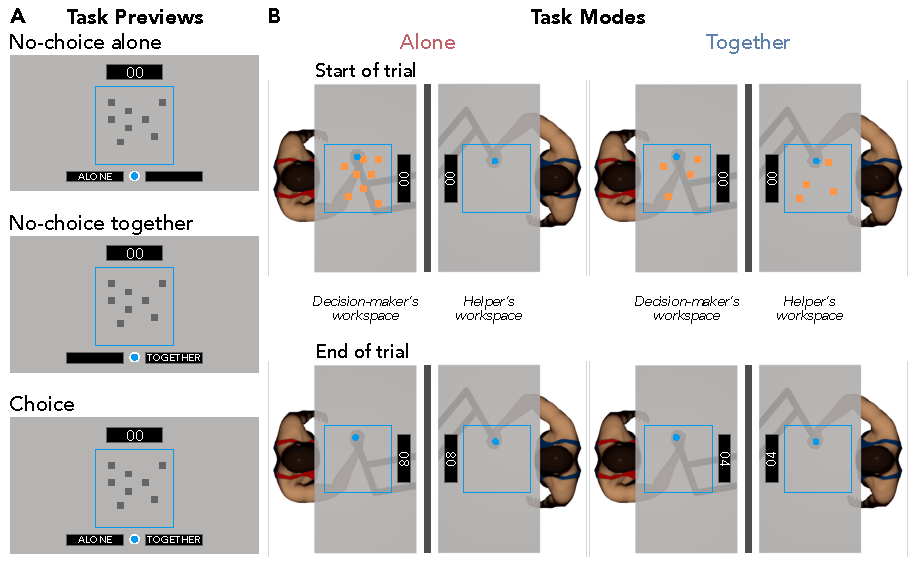
\includegraphics[scale=1.00]{../../figs/fig1.pdf}
\setlength{\belowcaptionskip}{-2em}
\caption*{\singlespacing \small Note. \normalfont Human pairs performed a virtual "box-clearing" task in either the Decision-maker role or the Helper role. \textbf{(A)} At the start of each trial, only the Decision-maker was shown a preview of the target box arrangement for the upcoming trial and two task mode selection boxes. In the no-choice trials, the Decision-maker was instructed to select the active task mode selection box (i.e., only one contained text) by moving their cursor into the box. In the choice trials, both task mode selection boxes were active and the Decision-maker was instructed to choose one of the two task modes. \textbf{(B)} Once a task mode was selected, the selection boxes disappeared and the target boxes changed colour from gray to orange. This change in colours served as the GO-signal for participants. In alone trials, all boxes shown in the preview remained in the Decision-maker's workspace while the Helper saw an empty workspace. In together trials, the boxes were evenly distributed across each participant's workspace and appeared in the same arrangement. Trials ended once all boxes were cleared or timed out after 100 s. One point per box was earned for boxes cleared by the Decision-maker.}
\label{fig:fig1}
\end{figure}

\clearpage

After participants completed all experimental trials, the
Decision-makers were asked a series of open-ended questions regarding
their decision-making processes. The Decision-makers answered these
questions by typing their responses in a survey form on a laptop that
were saved for later analysis. Participants were asked to answer the
following questions: a) ``When given the choice to do the task alone or
together with the Helper, \emph{why} did you choose to complete the task
\emph{alone}?'', b) ``When given the choice to do the task alone or
together with the Helper, \emph{when} did you choose to complete the
task \emph{alone}?'', c) ``When given the choice to do the task alone or
together with the Helper, \emph{why} did you choose to complete the task
\emph{together}?'', d) ``When given the choice to do the task alone or
together with the Helper, \emph{when} did you choose to complete the
task \emph{together}?'', and e) ``Is there anything else you would like
to tell us about how you completed the task?''. No follow-up questions
were asked regarding participants' responses. Participants required
approximately five minutes to complete this part of the experiment.

\subsection{Data analysis}\label{data-analysis}

\subsubsection{Choice data}\label{choice-data}

Our primary outcome variable was the proportion of trials in the choice
task mode where the Decision-makers selected to perform the task with
the Helper (i.e., to perform a joint rather than solo action). To gain
better insights into the reasons the Decision-makers used when choosing
to perform the task alone or together, we conducted an inductive
thematic content analysis (\citeproc{ref-braun2006}{Braun \& Clarke,
2006}) to identify, analyze, and report themes within the open-ended
questionnaire data. The analysis was conducted in a stepwise process.
First, the primary coder (M.L.) read through all participants' responses
to the open-ended questions and made initial notes of the content of the
data. This allowed the coder to become familiar with the data,
specifically the depth and breadth of the responses. Next, the coder
systematically worked through the entire data set, identifying segments
of responses (i.e., sentences, phrases, or individual words) that shared
similar ideas or topics. While identifying such segments, the coder
generated labels (initial codes) for each common idea or topic. The
coder then generated various levels of themes by considering how
different codes could be combined to support overarching themes. The
coder first consolidated the initial codes into initial themes. These
initial themes were further combined to form intermediate themes.
Finally, the intermediate themes were once more grouped into a final set
of higher order themes. The operational definition, an example of a
participant's response, and the number of responses for each higher
order theme can be found in Table~\ref{tbl-table1}.

To ensure the validity of the identified themes and a reliable portrayal
of the data by the primary coder, intercoder reliability was measured
during the thematic analysis process following the guidelines of
O'Connor and Joffe (\citeproc{ref-oconnor2020}{2020}). This process
involved comparing the agreement of coding between two coders. After
grouping the initial codes into five final themes, the primary coder
provided a comparison coder (J.T.) with a random selection of 50\% of
the codes, as well as a list of the five final themes and the respective
operational definitions. The comparison coder was instructed to sort
each code into one of the five themes to the best of their knowledge
using the theme names and definitions. A comparison analysis was
performed to determine intercoder reliability between coders, which
resulted in a Cohen's \(\kappa\) of .88. This value is larger than the
recommended minimum value of .80 (\citeproc{ref-hruschka2004}{Hruschka
et al., 2004}), suggesting strong intercoder reliability and confirming
that the primary coder accurately represented the data within the five
final themes.

\clearpage

\begin{landscape}

\begin{table}

{\caption{{The five final themes from the thematic analysis, as well as
their operational definitions, intermediate and initial themes if
applicable, and an example of a participant's
response.}{\label{tbl-table1}}}
\vspace{-20pt}}

\begin{longtable*}[t]{lllll}
\toprule

\bottomrule
\end{longtable*}

\end{table}

\vspace{-2.5em}

\begingroup\fontsize{10.5}{12.5}\selectfont

\begin{longtable*}[l]{>{\raggedright\arraybackslash}p{3cm}>{\raggedright\arraybackslash}p{6cm}>{\raggedright\arraybackslash}p{3cm}>{\raggedright\arraybackslash}p{2cm}>{\raggedright\arraybackslash}p{6cm}}
\toprule
\textbf{Final theme} & \textbf{Definition} & \textbf{Intermediate theme} & \textbf{Initial theme} & \textbf{Example}\\
\midrule
Chose actions with greater instrumental utility & Made decisions with the intention of reducing the time or energy needed to complete the task, and/or increasing the amount of points that could be earned. & Reduced instrumental costs & Maximized speed & "I decided to do all the optional tasks alone because I knew it would be faster..." (Participant 212)\\
\addlinespace
 &  &  & Minimized movement & "I attempted to complete the task in the most effective and quickest way, moving the handle with the shortest distance possible." (Participant 111)\\
\addlinespace
 &  & Reduced cognitive costs & Minimized decisions required & "I chose to do the task alone when there were many boxes that were far away from each other as I knew it would be difficult to choose the same boxes as the helper." (Participant 101)\\
\addlinespace
 &  &  & Minimized difficult coordination & "[I chose alone] because it was more reliable and gave more points, it eliminated the variable of having to depend on another person’s timing and thinking." (Participant 107)\\
\addlinespace
 &  & Minimized task constraints & Completed the task in the "easiest way" & "It was easier to complete the task alone" (Participant 404)\\
\addlinespace
 &  &  & Considered the spatial arrangement of the boxes & "[I chose together] when there was not as high of a concentration of squares, but also when they were in close proximity with each other." (Participant 203)\\
\addlinespace
 &  & Maximized instrumental rewards & NA & "I chose to complete the task alone when I realized that the number of points I got from working together was not as much as working alone." (Participant 412)\\
\addlinespace
Chose actions with greater social value & Made decisions that were motivated by enhancing their own and/or their partner's  experience & Maximized intrinsic rewards & NA & "I found it more fun and interesting when I had to complete the task together because you can see how similarly or differently you and your partner think and what each person's first instinct is." (Participant 312)\\
\addlinespace
 &  & Prosocial behaviour & Empathy & "[I chose together] because I felt bad for my partner if he was left with nothing to do" (Participant 102)\\
\addlinespace
 &  &  & Fairness & "I chose to do the task together when I had done a few trials alone. I thought that my partner would be upset if I did a bunch of the trials on my own just to achieve more points, so I would sometimes choose to do them with her to make it more fair." (Participant 410)\\
\addlinespace
Flexibility in decision strategy & Open to changing their decisions throughout the experiment & NA & NA & "There were some instances where I felt me and the helper changed the way we were slicing the squares to try to imitate each other..." (Participant 211)\\
\addlinespace
Planned movement path & Discussed their own individual directional patterns they typically moved in and/or the order they planned to clear boxes in & NA & NA & "I noticed I tended to hit the boxes in a circular motion starting from the one closest to me, moving outwards, then returning to the starting area." (Participant 309)\\
\addlinespace
Made reliable decisions & Made decisions knowing they could perform the task consistently well in that task mode & NA & NA & "[I chose alone] because it was more reliable and gave more points, it eliminated the variable of having to depend on another person's timing and thinking." (Participant 107)\\
\bottomrule
\end{longtable*}
\endgroup{}

\end{landscape}

\clearpage

\subsubsection{Box clearing data}\label{box-clearing-data}

Our second outcome variable was trial completion time for no-choice
trials, which was the interval of time between the boxes turning orange
and the last box being cleared. Our third outcome variable was distance
traveled for no-choice trials, which was the total distance that an
individual's cursor moved in the interval of time between the boxes
turning orange and the last box being cleared.

Alpha was set to .05 for all quantitative analyses, which are described
below. Corrected degrees of freedom using the Greenhouse-Geisser method
are always reported when appropriate. Generalized eta squared
\((\eta_{G}^{2})\) is reported as an effect size for all omnibus tests.
Post-hoc comparisons were performed using the Holm-Bonferroni approach
to adjust for multiple comparisons. Statistical analyses were conducted
using R (Version 4.4.2; \citeproc{ref-base}{R Core Team, 2024}) and the
R-packages \emph{afex} {[}Version 1.4.1; (\citeproc{ref-afex}{Singmann
et al., 2024}), \emph{easystats} (Version 0.7.4;
\citeproc{ref-easystats}{Lüdecke et al., 2022}), \emph{emmeans} (Version
1.10.7; \citeproc{ref-emmeans}{Lenth, 2025}), \emph{grateful} (Version
0.2.10; \citeproc{ref-grateful}{Rodriguez-Sanchez \& Jackson, 2023}),
\emph{here} (Version 1.0.1; \citeproc{ref-here}{Müller, 2020}),
\emph{Hmisc} (Version 5.2.2; \citeproc{ref-Hmisc}{Harrell Jr, 2025}),
\emph{kableExtra} (Version 1.4.0; \citeproc{ref-kableExtra}{Zhu, 2024}),
\emph{patchwork} (Version 1.3.0; \citeproc{ref-patchwork}{Pedersen,
2024}), \emph{rcompanion} (Version 2.4.36;
\citeproc{ref-rcompanion}{Mangiafico, 2024}), \emph{renv} (Version
1.1.0; \citeproc{ref-renv}{Ushey \& Wickham, 2025}), \emph{tidyverse}
(Version 2.0.0; \citeproc{ref-tidyverse}{Wickham et al., 2019}), and
\emph{waffle} (Version 1.0.2; \citeproc{ref-waffle}{Rudis \& Gandy,
2023}) were used in this project.

\section{Results}\label{results}

\subsection{Choice data}\label{choice-data-1}

Participants showed a slight preference of acting alone (\emph{M} =
0.56, \emph{SD} = 0.23) compared to joint action (see Figure
\ref{fig:fig2}A). A two-tailed Wilcoxon signed-rank test comparing the
mean proportion of together choices against a 50\% chance level was not
significant, \emph{V} = 472.5, \emph{p} = .112, \emph{r} = -.225, 95\%
CI {[}-.0.478, 0.068{]}.

\clearpage

\begin{figure}[htbp]
\caption{The proportion of selecting to perform the task together on choice trials and the frequency of the global themes underlying the decision process.}
\centering
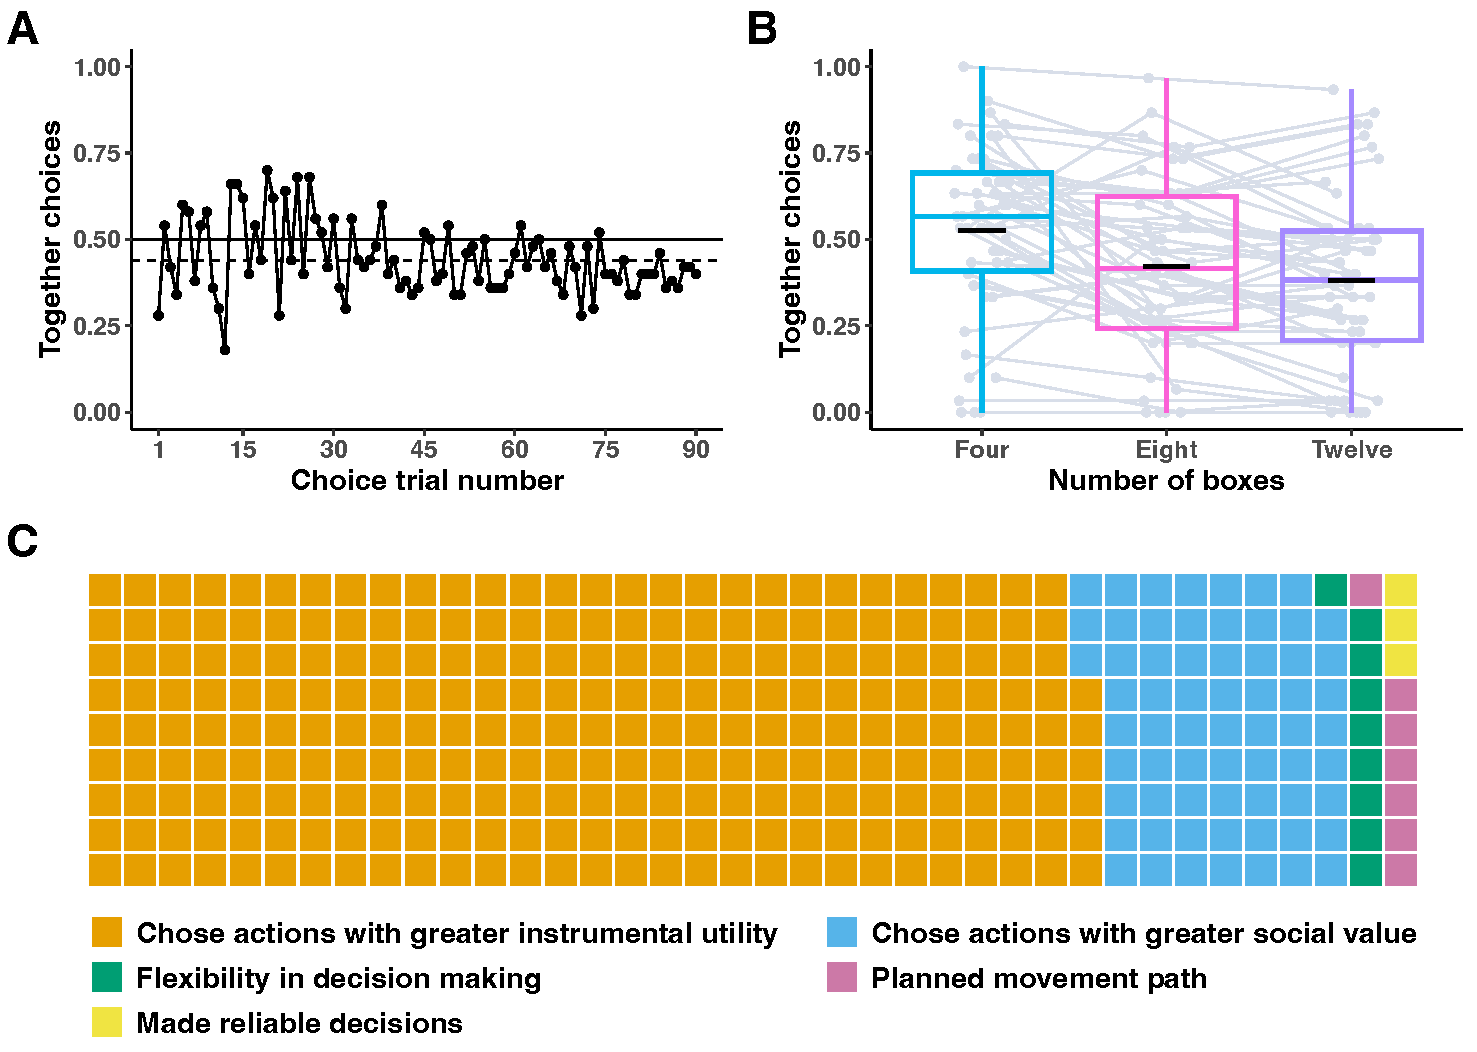
\includegraphics[scale=0.675]{../../figs/fig2.pdf}
\setlength{\belowcaptionskip}{-2em}
\caption*{\singlespacing \small Note. \normalfont During the experiment the Decision-maker could choose to perform the task either alone or together with their Helper on 90 choice trials. These choice trials were randomly interleaved with the forced alone and forced together trials. \textbf{(A)} The mean proportion of together choices across participants which is characterized by some early fluctuation that becomes more stable over trials. The solid and dashed horizontal lines represent the 50\% chance level and the mean of all choice trials, respectively. \textbf{(B)} Boxplots of the proportion of together choices as a function of the number of boxes on choice trials. Boxplots represent the 25th, 50th, and 75th percentiles, and the solid black line denotes the mean. Grey dots connected by grey lines represent means from individual participants. \textbf{(C)} Waffle plots showing the frequency of the five final themes based on the self-reported responses to the open-ended questions administered to the Decision-maker at the end of the experiment. Each square represents a code (single unit of information) aligning with one of the five final themes. The dominant theme was "chose actions with greater instrumental utility" (orange, *n* = 258) followed by "chose actions with greater social value" (blue, *n* = 65). The remaining themes were far less common.
}
\label{fig:fig2}
\end{figure}

\clearpage

We analyzed the proportion of together choices for each box number
condition (see Figure \ref{fig:fig2}B) using a one-way repeated measures
ANOVA. Participants chose to perform the task together more often when
there were fewer boxes to clear, \emph{F}(1.51, 74.06) = 16.43, \emph{p}
\textless{} .001, \(\eta_{G}^{2}\) = .057. The mean proportion of
together choices was greater for 4 boxes than all other numbers of boxes
(\emph{p's} \textless{} .002) and for 8 boxes than 12 boxes (\emph{p} =
.023).

Five final themes were identified (see Figure \ref{fig:fig2}C), which
represented participants' reasoning behind their decisions: ``chose
actions with greater instrumental utility'', ``chose actions with
greater social value'', ``made reliable decisions'', ``flexibility in
decision strategy'', and ``planned movement path''. The dominant
reasoning was ``chose actions with greater instrumental utility''
(\emph{n} = 258), followed by ``chose actions with greater social
value'' (\emph{n} = 65). The other three themes prevailed to similar
extents, with the least supported theme being ``made reliable
decisions'' (\emph{n} = 3).

The two most prominent themes were each composed of several intermediate
and initial themes. Within the first theme, ``chose actions with greater
instrumental utility'', participants expressed desires to: reduce
instrumental costs, reduce cognitive costs, minimize task constraints,
and maximize instrumental rewards. Reducing instrumental costs included
ideas of \emph{maximizing speed} and \emph{minimizing movement}, while
efforts to reduce cognitive costs included \emph{minimizing the amount
of decisions required} and \emph{minimizing difficult coordination}.
Participants minimized task constraints by \emph{completing the task in
the ``easiest'' way} and \emph{considering the spatial arrangement of
the boxes} as ways to prioritize efficiency and complete the task with
ease. These intermediate themes reflect the separate cost and reward
components of instrumental utility, and highlight the complexity of the
costs associated with action alternatives. For the second theme, ``chose
actions with greater social value'', participants reported making
efforts to: maximize intrinsic rewards and engage in prosocial
behaviour. Prosocial behaviours included acts of \emph{empathy} and
\emph{fairness}, taking the Helper's feelings or perspectives into
account, and choosing the task condition with the intention of being
inclusive to their partner.

\subsection{Box clearing data}\label{box-clearing-data-1}

We analyzed mean trial time (see Figure \ref{fig:fig3}A) using a 2 Task
Mode (Forced Alone, Forced Together) x 3 Number of Boxes (4, 8, 12)
repeated measures ANOVA. The significant main effects of Task Mode,
\emph{F}(1, 49) = 74.33, \emph{p} \textless{} .001, \(\eta_{G}^{2}\) =
.323, and Number of Boxes, \emph{F}(1.57, 76.85) = 266.51, \emph{p}
\textless{} .001, \(\eta_{G}^{2}\) = .422, were superseded by a
significant Task Mode × Number of Boxes interaction, \emph{F}(1.52,
74.57) = 56.57, \emph{p} \textless{} .001, \(\eta_{G}^{2}\) = .130. Post
hoc analyses revealed that participants were significantly faster at
performing the task alone than together with all number of boxes
(\emph{p}'s \textless{} .006), with 4 boxes than all other numbers of
boxes in both task modes (\emph{p}'s \textless{} .001), and with 8 boxes
than 12 boxes in both task modes (\emph{p}'s \textless{} .001).

To complement the trial time data we calculated the distance traveled in
each trial, with data from two representative participants for each task
mode and box conditions shown in Figure \ref{fig:fig3}C. We analyzed
mean distance traveled (see Figure \ref{fig:fig3}B) using a 2 Task Mode
(Alone, Together) x 3 Number of Boxes (4, 8, 12) repeated measures
ANOVA. The significant main effects of Task Mode, \emph{F}(1, 49) =
58.13, \emph{p} \textless{} .001, \(\eta_{G}^{2}\) = .255, and Number of
Boxes, \emph{F}(1.31, 64.22) = 370.88, \emph{p} \textless{} .001,
\(\eta_{G}^{2}\) = .577, were superseded by a significant Task Mode x
Number of Boxes interaction, \emph{F}(1.30, 63.69) = 62.23, \emph{p}
\textless{} .001, \(\eta_{G}^{2}\) = .173. Post hoc comparisons revealed
that participants traveled a significantly shorter distance when
performing the task alone than together with 8 and 12 boxes (\emph{p}'s
\textless{} .001), with 4 boxes than all other numbers of boxes in both
task modes (\emph{p}'s \textless{} .001), and with 8 boxes than 12 boxes
in both task modes (\emph{p}'s \textless{} .001).

\clearpage

\begin{figure}[htbp]
\caption{Trial time and distance traveled to clear boxes on forced alone and forced together trials.}
\centering
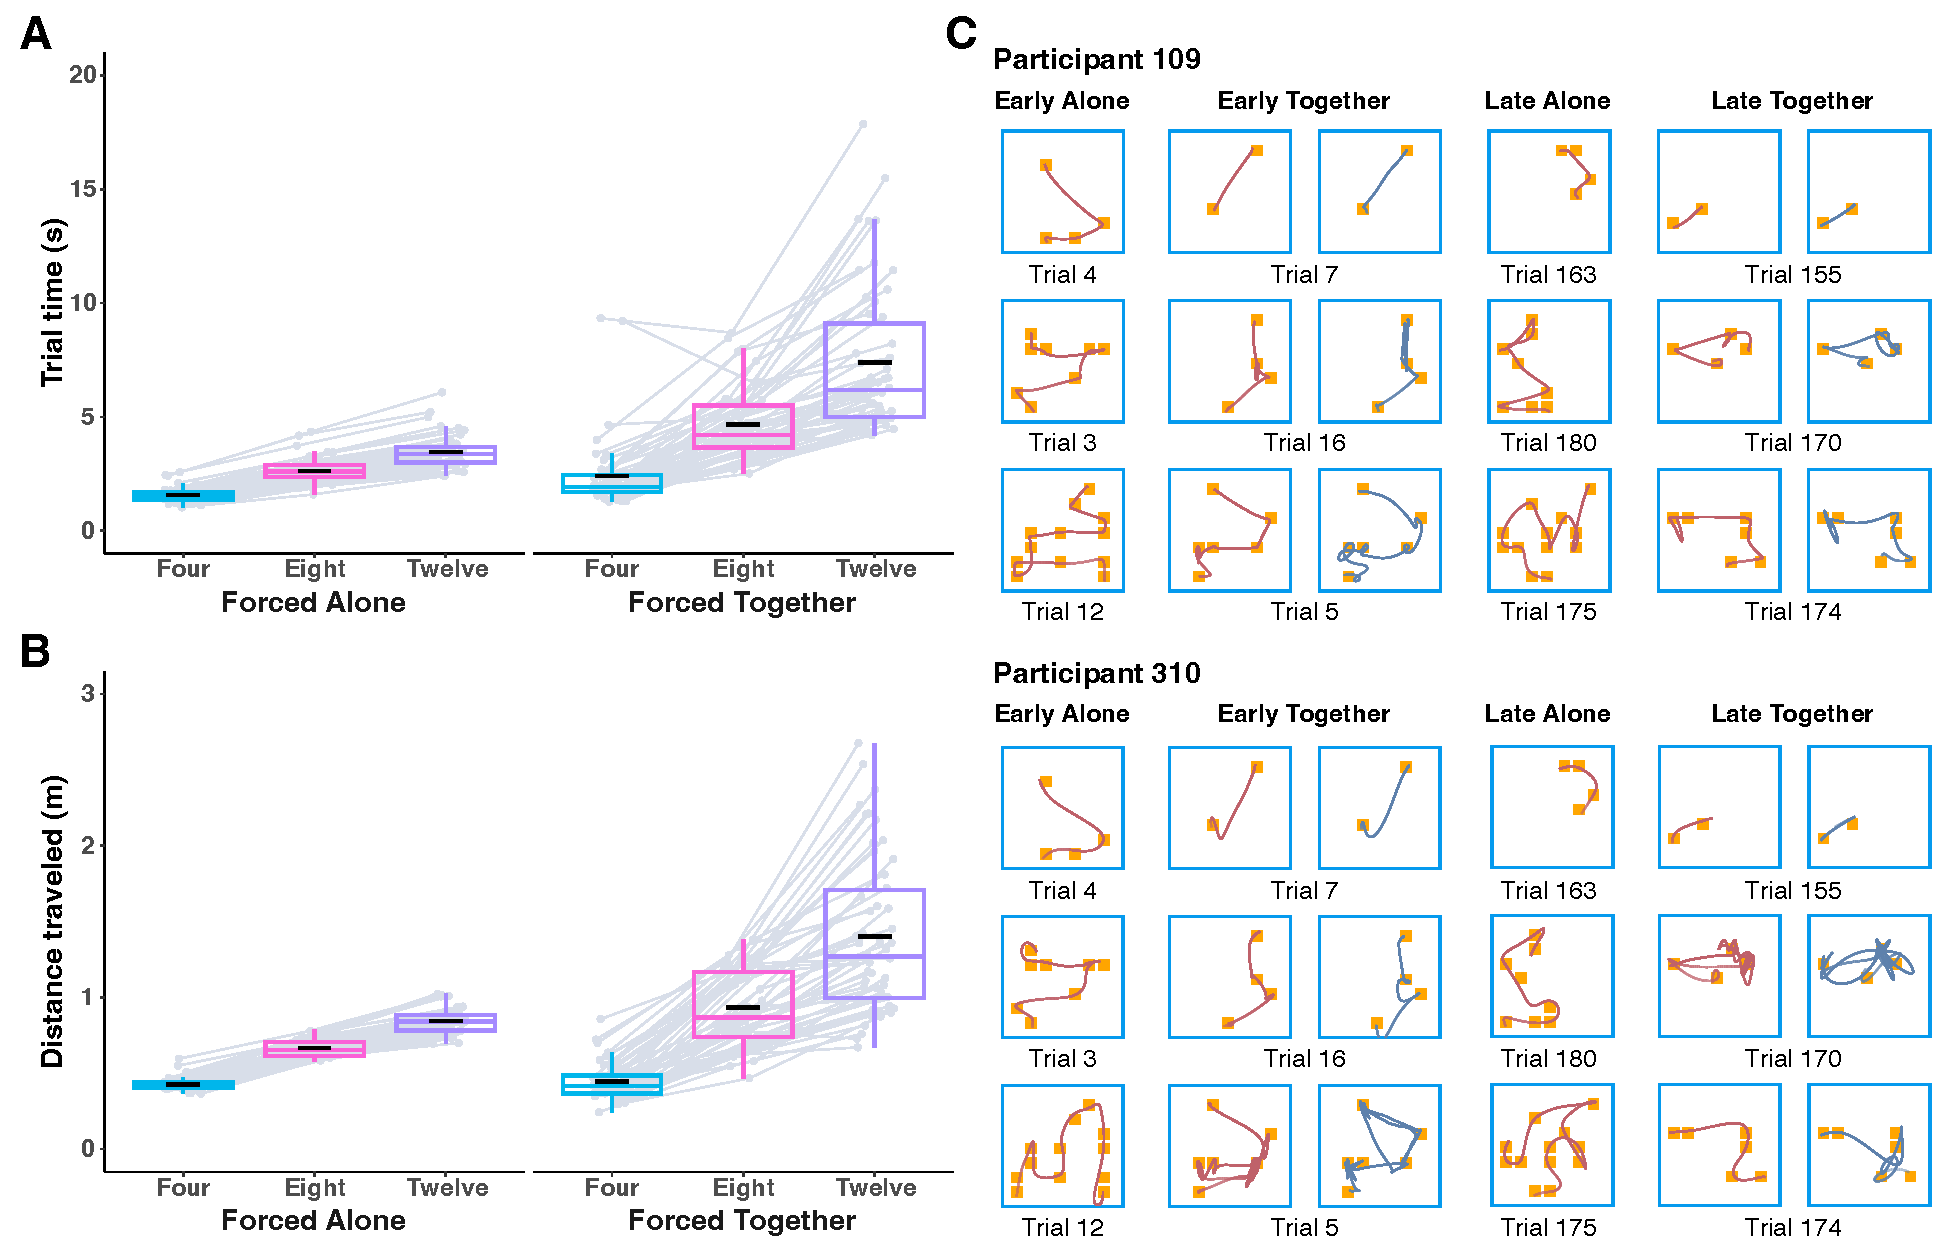
\includegraphics[scale=0.5]{../../figs/fig3.pdf}
\setlength{\belowcaptionskip}{-2em}
\caption*{\singlespacing \small Note. \normalfont \textbf{(A)} Boxplots of mean trial time (s), which was the interval of time between the boxes turning orange and the last box cleared, for each box condition in the forced alone and forced together trials. Participants were, on average, much faster when acting alone compared to together and not surprisingly, trial time increased as the number of boxes increased in both task modes. Boxplots represent the 25th, 50th, and 75th percentiles, and the solid black line denotes the mean. Grey dots connected by grey lines represent means from individual participants. \textbf{(B)} Boxplots of mean distance traveled (m), which was the total distance that a participant's cursor moved during the interval of time between the boxes turning orange and the last box cleared, for each box condition in the forced alone and forced together trials. Participants moved, on average, less when acting alone compared to together and distance traveled increased in both task modes as the number of boxes increased. Boxplots represent the 25th, 50th, and 75th percentiles, and the solid black line denotes the mean. Grey dots connected by grey lines represent means from individual participants. \textbf{(C)} Sample hand trajectory plots for two Decision-maker (red lines) and Helper (blue lines) participant pairs for early and late forced alone and force together trials for each box condition.
}
\label{fig:fig3}
\end{figure}

\clearpage

\section{Discussion}\label{discussion}

We found that participants showed a modest preference for solo action
over joint action, which is opposite to what Curioni et al.
(\citeproc{ref-curioni2022}{2022}) found. Although this preference for
solo action was not significantly different from chance levels, we did
find that these preferences varied considerably at the individual level
(range: 0.033\%-100\%). This was also evident from the participants'
responses on the open-ended questionnaire. Interestingly, the slight
preference we found for solo action over joint action is less than what
would be expected based solely on principles of utility and optimization
(\citeproc{ref-jara-ettinger2016}{Jara-Ettinger et al., 2016},
\citeproc{ref-jara-ettinger2020}{2020};
\citeproc{ref-shadmehr2016}{Shadmehr et al., 2016};
\citeproc{ref-todorov2004}{Todorov, 2004}). Thus, in line with Curioni
et al. (\citeproc{ref-curioni2022}{2022}), our findings suggest that
humans may assign additional reward value to performing actions with
another person.

Our failure to replicate a preference for joint action even when it is
more costly was surprising given the robustness of this effect across
multiple experiments in Curioni et al.
(\citeproc{ref-curioni2022}{2022}). Importantly, this difference cannot
be attributed to a failure on our part of not implementing a version of
the box-clearing task wherein performing the task together was both more
instrumentally costly and suboptimal. That is, less points could only
ever be earned on together trials and all Decision-makers were, on
average, significantly slower (see Figure \ref{fig:fig3}A) and made
significantly more movements (except in the 4 box arrangement; see
Figure \ref{fig:fig3}B) when performing the task together compared to
alone. In contrast, there was a small subset of participants in
Experiment 1 of Curioni et al. (\citeproc{ref-curioni2022}{2022}) that
were actually faster, on average, when performing the task with their
Helper compared to alone. One possibility is that it is this subset of
participants that drove the effect as these participants were able to
reduce their coordination costs and clear boxes more efficiently through
joint action. Based on the data from Experiment 4 of Curioni et al.
(\citeproc{ref-curioni2022}{2022}), we think this is an unlikely
explanation as the strong preference for joint action was found; yet,
similar to our data all Decision-makers, on average, were slower at
clearing boxes and covered more distance with their partner compared to
alone. We, instead, attribute our conflicting results to the differences
in the physical proximity of participants between studies. When human
pairs act on the same device beside one another, as in Curioni et al.
(\citeproc{ref-curioni2022}{2022}), it is very likely that the
Decision-makers experienced increased pressure to cooperate, presumably
through a desire to manage one's reputation
(\citeproc{ref-nowak2005}{Nowak \& Sigmund, 2005};
\citeproc{ref-wu2016}{Wu et al., 2016}) or a heightened sense of
commitment (\citeproc{ref-michael2016}{Michael et al., 2016a};
\citeproc{ref-michael2022}{Michael, 2022}). Merely positioning
participant pairs on separate devices and at a distance of approximately
3 m from each other flipped the effect to a small preference for solo
action (56\% in our experiment versus the 76\% preference for joint
action in Curioni et al. (\citeproc{ref-curioni2022}{2022})).
Nevertheless, participants in our experiment self-reported empathy
(e.g., \citeproc{ref-rumble2010}{Rumble et al., 2010}) and fairness
(e.g., \citeproc{ref-szekely2023}{Székely \& Michael, 2023}) as reasons
for choosing to perform the task with the Helper, suggesting that social
pressures to cooperate may have still been at play with our setup, but
to a lesser extent. Further research is needed to better understand the
influence of these social factors on the decision to engage, or not
engage, in joint action, such as having participants in separate rooms
akin to playing a game online or having participants perform the task in
both the Decision-maker and Helper roles.

Although the mean proportion of choosing solo trials across participants
was not significantly different from chance, there was considerable
variability between participants. In fact, a subset of participants
always chose to perform the task alone whereas one participant chose to
perform the task together on nearly every opportunity (see Figure
\ref{fig:fig2}B). We suggest that participants' choices were in fact not
random and instead reflect rather highly individualized preferences. In
support of this, our thematic analysis revealed that no participant
described making exclusively random or unrationalized decisions---each
participant self-reported at least one deliberate reason within their
responses. Thus, if some kind of generic additional reward value is
assigned to performing a task with another person, it may largely depend
on the individual and/or socio-cultural and psychological variables not
explored in the current experiment. Motivation measures, such as the
Balanced Inventory of Desirable Responding
(\citeproc{ref-paulhus1998}{Paulhus, 1998}) or the Ring Measure of
Social Values (\citeproc{ref-liebrand1988}{Liebrand \& McClintock,
1988}), as well as personality inventories and other validated scales
that assess individual differences could be implemented in future
research to better understand the intersectionality of these factors
(\citeproc{ref-appelt2011}{Appelt et al., 2011}).

The most prominent higher order theme identified through our thematic
analysis was ``chose actions with greater instrumental utility'' (see
Figure \ref{fig:fig2}C). The sub themes within this category revealed
that the Decision-makers were mindful of the task goal (i.e., earn as
many points as possible) and often aimed to maximize the utility of
their actions when making their decisions. Participants frequently
reported wanting to complete the task in the fastest way (overwhelmingly
perceived to be the alone condition) or choosing the task condition they
thought would require the least amount of movement. This behaviour
aligns with the Naive Utility Calculus
(\citeproc{ref-jara-ettinger2016}{Jara-Ettinger et al., 2016},
\citeproc{ref-jara-ettinger2020}{2020}); however, if these participants
exclusively considered the instrumental factors of the action
alternatives (e.g., points earned, time spent, actions required, etc),
we would expect to see a much greater proportion of alone trials than we
observed in the choice trials. Many participants also described choosing
to work together when there were fewer boxes to clear as they perceived
the task to be easier compared to when there were more boxes. With more
boxes, participants described it would not only be difficult to select
the same box as the Helper, but also coordinate their movements more
times. In line with this, we did find that participants made
significantly less together choices as the number of boxes to clear
increased. Being able to predict an interaction partner's behaviour is
an important mechanism for successful coordination
(\citeproc{ref-sebanz2006}{Sebanz et al., 2006}). Although the identical
arrangement of boxes in each workspace would allow partners to share
representations of the task, the unspecified order that the boxes could
be cleared made it difficult for participants to predict each other's
movement path. Future work should focus on the relationship between
individual costs and joint costs during joint action.

Despite the abundance of utility-centered participant responses in our
thematic analysis, our data, together with that of Curioni and
colleagues (\citeproc{ref-curioni2022}{2022}), strongly suggest that
other factors currently unaccounted for in the utility calculus may
outweigh instrumental factors and motivate individuals to engage in
costly joint action even when it is unnecessary. This could be
represented by a \emph{cooperation reward} variable in the calculus
(\citeproc{ref-curioni2022}{Curioni et al., 2022}); an idea that is
supported by our second prominent theme of ``chose actions with greater
social value''. For example, participants described working together as
being intrinsically rewarding and that they felt motivated by the
enjoyment and enrichment they experienced from the added challenge of
coordinating. Others acknowledged the prosocial benefits
(\citeproc{ref-eisenberg2015}{Eisenberg et al., 2015}) associated with
choosing to perform the task together with their partner (e.g.,
\citeproc{ref-michael2020}{Michael et al., 2020};
\citeproc{ref-obhi2011}{Obhi \& Sebanz, 2011};
\citeproc{ref-vanderwel2021}{van der Wel et al., 2021}). These
individuals empathized with the Helper, choosing together when they felt
bad that their partner was left doing nothing or had not participated in
a while. This resulted in some participants balancing the distribution
of alone and together trials throughout the experiment as a way to be
fair towards their partner. Interestingly, these participants did
acknowledge that they incurred additional costs and reduced
(instrumental) benefits by working together; therefore, the value
derived from making the task more fair was oftentimes strong enough to
offset the weight of the instrumental factors in the task.

A possible limitation of our experiment is our use of a convenience
sample of undergraduate students; thus, some participant pairs may have
already been familiar with one another compared to others, or complete
strangers. Individuals may be more inclined to interact with people they
know or have previously had positive experiences working with
(\citeproc{ref-hinds2000}{Hinds et al., 2000};
\citeproc{ref-zander1960}{Zander \& Havelin, 1960}), as a means to
increase the predictability of others' actions. Similar to Curioni et
al. (\citeproc{ref-curioni2022}{2022}), our participant pairs were
created randomly without controlling for sex, gender, age, or ethnicity.
Demographics and identification with co-actors have been shown to impact
decisions to cooperate (\citeproc{ref-chen2012}{Chen et al., 2012};
e.g., \citeproc{ref-chuah2014}{Chuah et al., 2014};
\citeproc{ref-krumhuber2007}{Krumhuber et al., 2007};
\citeproc{ref-levy2004}{Levy et al., 2004}), ability to coordinate
(\citeproc{ref-boukarras2021}{Boukarras et al., 2021}), and partner
choice in interactive tasks (\citeproc{ref-chuah2014}{Chuah et al.,
2014}; \citeproc{ref-krumhuber2007}{Krumhuber et al., 2007}). Exploring
the influence of these factors in future research may have important
practical implications, especially in workplace settings.

In conclusion, we did not find a strong preference for costly
cooperative action like that observed by Curioni et al.
(\citeproc{ref-curioni2022}{2022}). Instead, we found a slight
preference for choosing individual action, but this was much lower than
would be expected if these choices were solely guided by principles of
optimization and utility. Our quantitative and qualitative data add
further support to the idea that additional rewards are derived from the
social nature of joint action (e.g., \citeproc{ref-curioni2022}{Curioni
et al., 2022}) and that these preferences are highly individualized.

\vfill

\section{Declarations}\label{declarations}

\noindent \textbf{Funding.} \space This work was supported by
{[}anonymized source{]}, {[}anonymized source{]}, and {[}anonymized
source{]}.

\noindent \textbf{Conflicts of interest/Competing interests.}
\space None.

\noindent \textbf{Ethics approval.} \space This project was approved and
conducted in accordance with the approval of the University's Research
Ethics Board.

\noindent \textbf{Consent to participate.} \space All participants gave
informed consent.

\noindent \textbf{Consent for publication.} \space All authors approve
the manuscript.

\noindent \textbf{Availability of data, materials, and code.}
\space Available at
\url{https://osf.io/fq3mz/?view_only=8dffee7f8b364159b30ec8527ee0c498}.

\newpage

\section{References}\label{references}

\phantomsection\label{refs}
\begin{CSLReferences}{1}{0}
\bibitem[\citeproctext]{ref-appelt2011}
Appelt, K. C., Milch, K. F., Handgraaf, M. J. J., \& Weber, E. U.
(2011). The {Decision Making Individual Differences Inventory} and
guidelines for the study of individual differences in judgment and
decision-making research. \emph{Judgment and Decision Making},
\emph{6}(3), 252--262. \url{https://doi.org/10.1017/S1930297500001455}

\bibitem[\citeproctext]{ref-boukarras2021}
Boukarras, S., Era, V., Aglioti, S. M., \& Candidi, M. (2021).
Competence-based social status and implicit preference modulate the
ability to coordinate during a joint grasping task. \emph{Scientific
Reports}, \emph{11}(1), 5321.
\url{https://doi.org/10.1038/s41598-021-84280-z}

\bibitem[\citeproctext]{ref-braun2006}
Braun, V., \& Clarke, V. (2006). Using thematic analysis in psychology.
\emph{Qualitative Research in Psychology}, \emph{3}(2), 77--101.

\bibitem[\citeproctext]{ref-chen2012}
Chen, J., Zhong, J., Zhang, Y., Li, P., Zhang, A., Tan, Q., \& Li, H.
(2012). Electrophysiological correlates of processing facial
attractiveness and its influence on cooperative behavior.
\emph{Neuroscience Letters}, \emph{517}(2), 65--70.
\url{https://doi.org/10.1016/j.neulet.2012.02.082}

\bibitem[\citeproctext]{ref-chuah2014}
Chuah, S.-H., Hoffmann, R., Ramasamy, B., \& Tan, J. H. (2014).
Religion, ethnicity and cooperation: {An} experimental study.
\emph{Journal of Economic Psychology}, \emph{45}, 33--43.

\bibitem[\citeproctext]{ref-cos2011}
Cos, I., Bélanger, N., \& Cisek, P. (2011). The influence of predicted
arm biomechanics on decision making. \emph{Journal of Neurophysiology},
\emph{105}(6), 3022--3033. \url{https://doi.org/10.1152/jn.00975.2010}

\bibitem[\citeproctext]{ref-cos2014}
Cos, I., Duque, J., \& Cisek, P. (2014). Rapid prediction of
biomechanical costs during action decisions. \emph{Journal of
Neurophysiology}, \emph{112}(6), 1256--1266.
\url{https://doi.org/10.1152/jn.00147.2014}

\bibitem[\citeproctext]{ref-curioni2022}
Curioni, A., Voinov, P., Allritz, M., Wolf, T., Call, J., \& Knoblich,
G. (2022). Human adults prefer to cooperate even when it is costly.
\emph{Proceedings of the Royal Society B: Biological Sciences},
\emph{289}(1973), 20220128. \url{https://doi.org/10.1098/rspb.2022.0128}

\bibitem[\citeproctext]{ref-eisenberg2015}
Eisenberg, N., Eggum, N. D., \& Spinrad, T. L. (2015). {114The
Development} of {Prosocial Behavior}. In D. A. Schroeder \& W. G.
Graziano (Eds.), \emph{The {Oxford Handbook} of {Prosocial Behavior}}
(p. 0). Oxford University Press.
\url{https://doi.org/10.1093/oxfordhb/9780195399813.013.008}

\bibitem[\citeproctext]{ref-gallivan2018}
Gallivan, J. P., Chapman, C. S., Wolpert, D. M., \& Flanagan, J. R.
(2018). Decision-making in sensorimotor control. \emph{Nature Reviews
Neuroscience}, \emph{19}(9), 519--534.
\url{https://doi.org/10.1038/s41583-018-0045-9}

\bibitem[\citeproctext]{ref-gordon2021}
Gordon, J., Maselli, A., Lancia, G. L., Thiery, T., Cisek, P., \&
Pezzulo, G. (2021). The road towards understanding embodied decisions.
\emph{Neuroscience \& Biobehavioral Reviews}, \emph{131}, 722--736.
\url{https://doi.org/10.1016/j.neubiorev.2021.09.034}

\bibitem[\citeproctext]{ref-Hmisc}
Harrell Jr, F. E. (2025). \emph{{Hmisc}: Harrell miscellaneous}.
\url{https://CRAN.R-project.org/package=Hmisc}

\bibitem[\citeproctext]{ref-hinds2000}
Hinds, P. J., Carley, K. M., Krackhardt, D., \& Wholey, D. (2000).
Choosing {Work Group Members}: {Balancing Similarity}, {Competence}, and
{Familiarity}. \emph{Organizational Behavior and Human Decision
Processes}, \emph{81}(2), 226--251.
\url{https://doi.org/10.1006/obhd.1999.2875}

\bibitem[\citeproctext]{ref-hruschka2004}
Hruschka, D. J., Schwartz, D., St.John, D. C., Picone-Decaro, E.,
Jenkins, R. A., \& Carey, J. W. (2004). Reliability in {Coding
Open-Ended Data}: {Lessons Learned} from {HIV Behavioral Research}.
\emph{Field Methods}, \emph{16}(3), 307--331.
\url{https://doi.org/10.1177/1525822X04266540}

\bibitem[\citeproctext]{ref-jara-ettinger2016}
Jara-Ettinger, J., Gweon, H., Schulz, L. E., \& Tenenbaum, J. B. (2016).
The {Na{ï}ve Utility Calculus}: {Computational Principles Underlying
Commonsense Psychology}. \emph{Trends in Cognitive Sciences},
\emph{20}(8), 589--604. \url{https://doi.org/10.1016/j.tics.2016.05.011}

\bibitem[\citeproctext]{ref-jara-ettinger2020}
Jara-Ettinger, J., Schulz, L. E., \& Tenenbaum, J. B. (2020). The
{Na{ï}ve Utility Calculus} as a unified, quantitative framework for
action understanding. \emph{Cognitive Psychology}, \emph{123}, 101334.
\url{https://doi.org/10.1016/j.cogpsych.2020.101334}

\bibitem[\citeproctext]{ref-kahneman2012}
Kahneman, D., \& Tversky, A. (2012). Prospect {Theory}: {An Analysis} of
{Decision Under Risk}. In \emph{Handbook of the {Fundamentals} of
{Financial Decision Making}: Vols. Volume 4} (pp. 99--127). WORLD
SCIENTIFIC. \url{https://doi.org/10.1142/9789814417358_0006}

\bibitem[\citeproctext]{ref-knoblich2011}
Knoblich, G., Butterfill, S., \& Sebanz, N. (2011). Psychological
research on joint action: Theory and data. \emph{Psychology of Learning
and Motivation}, \emph{54}, 59--101.

\bibitem[\citeproctext]{ref-kourtis2014}
Kourtis, D., Knoblich, G., Woźniak, M., \& Sebanz, N. (2014). Attention
{Allocation} and {Task Representation} during {Joint Action Planning}.
\emph{Journal of Cognitive Neuroscience}, \emph{26}(10), 2275--2286.
\url{https://doi.org/10.1162/jocn_a_00634}

\bibitem[\citeproctext]{ref-krumhuber2007}
Krumhuber, E., Manstead, A. S., Cosker, D., Marshall, D., Rosin, P. L.,
\& Kappas, A. (2007). Facial dynamics as indicators of trustworthiness
and cooperative behavior. \emph{Emotion}, \emph{7}(4), 730.

\bibitem[\citeproctext]{ref-emmeans}
Lenth, R. V. (2025). \emph{{emmeans}: Estimated marginal means, aka
least-squares means}. \url{https://CRAN.R-project.org/package=emmeans}

\bibitem[\citeproctext]{ref-levy2004}
Levy, I., Kaplan, A., \& Patrick, H. (2004). Early {Adolescents}'
{Achievement Goals}, {Social Status}, and {Attitudes Towards
Cooperation} with {Peers}. \emph{Social Psychology of Education},
\emph{7}(2), 127--159.
\url{https://doi.org/10.1023/B:SPOE.0000018547.08294.b6}

\bibitem[\citeproctext]{ref-liebrand1988}
Liebrand, W. B., \& McClintock, C. G. (1988). The ring measure of social
values: {A} computerized procedure for assessing individual differences
in information processing and social value orientation. \emph{European
Journal of Personality}, \emph{2}(3), 217--230.

\bibitem[\citeproctext]{ref-easystats}
Lüdecke, D., Ben-Shachar, M. S., Patil, I., Wiernik, B. M., Bacher, E.,
Thériault, R., \& Makowski, D. (2022). {easystats}: Framework for easy
statistical modeling, visualization, and reporting. \emph{CRAN}.
\url{https://doi.org/10.32614/CRAN.package.easystats}

\bibitem[\citeproctext]{ref-rcompanion}
Mangiafico, S. S. (2024). \emph{{rcompanion}: Functions to support
extension education program evaluation}. Rutgers Cooperative Extension.
\url{https://CRAN.R-project.org/package=rcompanion/}

\bibitem[\citeproctext]{ref-michael2022}
Michael, J. (2022). \emph{The philosophy and psychology of commitment}.
Taylor \& Francis.

\bibitem[\citeproctext]{ref-michael2020}
Michael, J., McEllin, L., \& Felber, A. (2020). Prosocial effects of
coordination -- {What}, how and why? \emph{Acta Psychologica},
\emph{207}, 103083. \url{https://doi.org/10.1016/j.actpsy.2020.103083}

\bibitem[\citeproctext]{ref-michael2016}
Michael, J., Sebanz, N., \& Knoblich, G. (2016a). Observing joint
action: {Coordination} creates commitment. \emph{Cognition}, \emph{157},
106--113. \url{https://doi.org/10.1016/j.cognition.2016.08.024}

\bibitem[\citeproctext]{ref-michael2016a}
Michael, J., Sebanz, N., \& Knoblich, G. (2016b). The {Sense} of
{Commitment}: {A Minimal Approach}. \emph{Frontiers in Psychology},
\emph{6}.

\bibitem[\citeproctext]{ref-moskowitz2023}
Moskowitz, J. B., Berger, S. A., Fooken, J., Castelhano, M. S.,
Gallivan, J. P., \& Flanagan, J. R. (2023). The influence of
movement-related costs when searching to act and acting to search.
\emph{Journal of Neurophysiology}, \emph{129}(1), 115--130.
\url{https://doi.org/10.1152/jn.00305.2022}

\bibitem[\citeproctext]{ref-mosteller1951}
Mosteller, F., \& Nogee, P. (1951). An {Experimental Measurement} of
{Utility}. \emph{Journal of Political Economy}, \emph{59}(5), 371--404.
\url{https://www.jstor.org/stable/1825254}

\bibitem[\citeproctext]{ref-here}
Müller, K. (2020). \emph{{here}: A simpler way to find your files}.
\url{https://CRAN.R-project.org/package=here}

\bibitem[\citeproctext]{ref-nowak2005}
Nowak, M. A., \& Sigmund, K. (2005). Evolution of indirect reciprocity.
\emph{Nature}, \emph{437}(7063), 1291--1298.
\url{https://doi.org/10.1038/nature04131}

\bibitem[\citeproctext]{ref-oconnor2020}
O'Connor, C., \& Joffe, H. (2020). Intercoder {Reliability} in
{Qualitative Research}: {Debates} and {Practical Guidelines}.
\emph{International Journal of Qualitative Methods}, \emph{19},
1609406919899220. \url{https://doi.org/10.1177/1609406919899220}

\bibitem[\citeproctext]{ref-obhi2011}
Obhi, S. S., \& Sebanz, N. (2011). Moving together: Toward understanding
the mechanisms of joint action. \emph{Experimental Brain Research},
\emph{211}(3), 329--336. \url{https://doi.org/10.1007/s00221-011-2721-0}

\bibitem[\citeproctext]{ref-paulhus1998}
Paulhus, D. L. (1998). Balanced inventory of desirable responding.
\emph{Journal of Personality and Social Psychology}.

\bibitem[\citeproctext]{ref-patchwork}
Pedersen, T. L. (2024). \emph{{patchwork}: The composer of plots}.
\url{https://CRAN.R-project.org/package=patchwork}

\bibitem[\citeproctext]{ref-base}
R Core Team. (2024). \emph{{R}: A language and environment for
statistical computing}. R Foundation for Statistical Computing.
\url{https://www.R-project.org/}

\bibitem[\citeproctext]{ref-rangel2008}
Rangel, A., Camerer, C., \& Montague, P. R. (2008). A framework for
studying the neurobiology of value-based decision making. \emph{Nature
Reviews Neuroscience}, \emph{9}(7), 545--556.
\url{https://doi.org/10.1038/nrn2357}

\bibitem[\citeproctext]{ref-grateful}
Rodriguez-Sanchez, F., \& Jackson, C. P. (2023). \emph{{grateful}:
Facilitate citation of r packages}.
\url{https://pakillo.github.io/grateful/}

\bibitem[\citeproctext]{ref-waffle}
Rudis, B., \& Gandy, D. (2023). \emph{{waffle}: Create waffle chart
visualizations}. \url{https://CRAN.R-project.org/package=waffle}

\bibitem[\citeproctext]{ref-rumble2010}
Rumble, A. C., Van Lange, P. A., \& Parks, C. D. (2010). The benefits of
empathy: {When} empathy may sustain cooperation in social dilemmas.
\emph{European Journal of Social Psychology}, \emph{40}(5), 856--866.

\bibitem[\citeproctext]{ref-schmidt2008}
Schmidt, R. C., \& Richardson, M. J. (2008). Dynamics of interpersonal
coordination. \emph{Coordination: Neural, Behavioral and Social
Dynamics}, 281--308.

\bibitem[\citeproctext]{ref-sebanz2006}
Sebanz, N., Bekkering, H., \& Knoblich, G. (2006). Joint action: Bodies
and minds moving together. \emph{Trends in Cognitive Sciences},
\emph{10}(2), 70--76. \url{https://doi.org/10.1016/j.tics.2005.12.009}

\bibitem[\citeproctext]{ref-sebanz2021}
Sebanz, N., \& Knoblich, G. (2021). Progress in {Joint-Action Research}.
\emph{Current Directions in Psychological Science}, \emph{30}(2),
138--143. \url{https://doi.org/10.1177/0963721420984425}

\bibitem[\citeproctext]{ref-shadmehr2016}
Shadmehr, R., Huang, H. J., \& Ahmed, A. A. (2016). A {Representation}
of {Effort} in {Decision-Making} and {Motor Control}. \emph{Current
Biology}, \emph{26}(14), 1929--1934.
\url{https://doi.org/10.1016/j.cub.2016.05.065}

\bibitem[\citeproctext]{ref-simmons2012}
Simmons, J. P., Nelson, L. D., \& Simonsohn, U. (2012). A 21 word
solution. \emph{Available at SSRN 2160588}.

\bibitem[\citeproctext]{ref-simonsohn2015}
Simonsohn, U. (2015). Small {Telescopes}: {Detectability} and the
{Evaluation} of {Replication Results}. \emph{Psychological Science},
\emph{26}(5), 559--569. \url{https://doi.org/10.1177/0956797614567341}

\bibitem[\citeproctext]{ref-afex}
Singmann, H., Bolker, B., Westfall, J., Aust, F., \& Ben-Shachar, M. S.
(2024). \emph{{afex}: Analysis of factorial experiments}.
\url{https://CRAN.R-project.org/package=afex}

\bibitem[\citeproctext]{ref-szekely2023}
Székely, M., \& Michael, J. (2023). In it together: {Evidence} of a
preference for the fair distribution of effort in joint action.
\emph{Evolution and Human Behavior}, \emph{44}(4), 339--348.

\bibitem[\citeproctext]{ref-todorov2004}
Todorov, E. (2004). Optimality principles in sensorimotor control.
\emph{Nature Neuroscience}, \emph{7}(9), 907--915.
\url{https://doi.org/10.1038/nn1309}

\bibitem[\citeproctext]{ref-renv}
Ushey, K., \& Wickham, H. (2025). \emph{{renv}: Project environments}.
\url{https://CRAN.R-project.org/package=renv}

\bibitem[\citeproctext]{ref-vanderwel2021}
van der Wel, R. P. R. D., Becchio, C., Curioni, A., \& Wolf, T. (2021).
Understanding joint action: {Current} theoretical and empirical
approaches. \emph{Acta Psychologica}, \emph{215}, 103285.
\url{https://doi.org/10.1016/j.actpsy.2021.103285}

\bibitem[\citeproctext]{ref-tidyverse}
Wickham, H., Averick, M., Bryan, J., Chang, W., McGowan, L. D.,
François, R., Grolemund, G., Hayes, A., Henry, L., Hester, J., Kuhn, M.,
Pedersen, T. L., Miller, E., Bache, S. M., Müller, K., Ooms, J.,
Robinson, D., Seidel, D. P., Spinu, V., \ldots{} Yutani, H. (2019).
Welcome to the {tidyverse}. \emph{Journal of Open Source Software},
\emph{4}(43), 1686. \url{https://doi.org/10.21105/joss.01686}

\bibitem[\citeproctext]{ref-wu2016}
Wu, J., Balliet, D., \& Van Lange, P. A. (2016). Reputation, gossip, and
human cooperation. \emph{Social and Personality Psychology Compass},
\emph{10}(6), 350--364.

\bibitem[\citeproctext]{ref-zander1960}
Zander, A., \& Havelin, A. (1960). Social comparison and interpersonal
attraction. \emph{Human Relations}, \emph{13}(1), 21--32.

\bibitem[\citeproctext]{ref-kableExtra}
Zhu, H. (2024). \emph{{kableExtra}: Construct complex table with
{``{kable}''} and pipe syntax}.
\url{https://CRAN.R-project.org/package=kableExtra}

\end{CSLReferences}






\end{document}
